\documentclass[conference]{IEEEtran}
\IEEEoverridecommandlockouts
\usepackage{amsmath,amssymb,amsthm}
\usepackage{graphicx}
\usepackage{booktabs}
\usepackage{multirow}
\usepackage{url}
\usepackage{tikz}
\usetikzlibrary{arrows.meta,positioning,fit,calc}
\usepackage{balance}
\usepackage{microtype}
\usepackage{cite}
\usepackage{algorithm}
\usepackage{algpseudocode}
\makeatletter
\renewcommand{\ALG@name}{Algorithm}
\makeatother
\algrenewcommand\algorithmicrequire{\textbf{Input:}}
\algrenewcommand\algorithmicensure{\textbf{Output:}}

\newtheorem{proposition}{Proposition}
\DeclareMathOperator*{\argmin}{arg\,min}
\DeclareMathOperator*{\argmax}{arg\,max}

\begin{document}

\title{AI-Powered Unified Mobility and Delivery System\\ Using Dynamic Feasibility Analysis}

\author{%
\begin{minipage}{0.48\linewidth}\centering
Sivasubramanian M\\
\textit{Dept.\ of Computer Science and Engineering}\\
\textit{Dr.\ N.G.P.\ Institute of Technology}\\
Coimbatore, Tamil Nadu, India\\
sivamah25@gmail.com
\end{minipage}%
\begin{minipage}{0.48\linewidth}\centering
S.\ R.\ Ramya\\
\textit{Assistant Professor/CSE}\\
\textit{Dept.\ of Computer Science and Engineering}\\
\textit{Dr.\ N.G.P.\ Institute of Technology}\\
Coimbatore, Tamil Nadu, India\\
srramyacse@gmail.com
\end{minipage}%
\\[1.0em]
\begin{minipage}{0.48\linewidth}\centering
Rakshana S\\
\textit{Dept.\ of Computer Science and Engineering}\\
\textit{Dr.\ N.G.P.\ Institute of Technology}\\
Coimbatore, Tamil Nadu, India\\
rakshanasanjith05@gmail.com
\end{minipage}%
\begin{minipage}{0.48\linewidth}\centering
Sadhana T\\
\textit{Dept.\ of Computer Science and Engineering}\\
\textit{Dr.\ N.G.P.\ Institute of Technology}\\
Coimbatore, Tamil Nadu, India\\
sadhanathangamuthu16@gmail.com
\end{minipage}%
}

\maketitle

\begin{abstract}
Ride-hailing, food delivery and parcel courier platforms move vehicles over the same street network but plan in isolation, so three vehicles are often dispatched where one coordinated trip would do. This paper presents a unified pipeline built around a Dynamic Multi-Service Feasibility Engine (DMFE), which decides whether a passenger ride, a food order and a parcel drop can share a vehicle before any driver is committed or any route is planned. Candidate pairs are scored on pickup proximity, route similarity, time-window overlap, vehicle capacity and request priority; admitted batches are assigned by a five-factor driver selector and then routed by a constraint solver. An adaptive mode recomputes the scoring weights each dispatch cycle from operating context and from bounded corrections derived from completed-trip residuals. Evaluation used reproducible synthetic workloads of 50, 100, 250 and 500 requests over 36 seed-matched runs with a fixed 60-vehicle fleet, against an independent-dispatch baseline. Where both configurations served the same requests, batching cut dispatched trips by 36.8\% and 40.4\% and raised mean vehicle utilisation by 17.0 and 17.4 percentage points, at mean service delays of 5.8 and 6.1 minutes against a 20-minute cap. Consolidation within the assigned fleet lowered estimated CO$_2$ by 22.0\% to 43.9\% against serving the same requests unbatched. The adaptive mode improved consolidation at every workload and raised mean pair compatibility from 55.4 to 59.2. The evaluation is synthetic and single-region. The adaptive layer utilizes a bounded residual correction, which was empirically validated to improve batch compatibility. The gradient-based learning formulation is a proposed extension.
\end{abstract}

\begin{IEEEkeywords}
Adaptive systems, dynamic feasibility analysis, food delivery, parcel delivery, ride sharing, route optimisation, unified mobility, vehicle routing.
\end{IEEEkeywords}

\section{Introduction}
\subsection{Background and Motivation}
Three parallel economies now run over one street network. A passenger opens a ride-hailing app, a diner opens a food-delivery app, a shopper books a courier, and each of those requests is matched, routed and closed out inside a platform that cannot see the other two. At peak hour the predictable consequence is three vehicles from three operators working the same two blocks minutes apart, each carrying one job.

The waste is not a failure of any individual matching algorithm. It follows from treating passenger mobility, food delivery and parcel logistics as separate problems, when, to a road network, they are one flow of vehicle movements under three commercial labels. Shareability analysis of city-scale taxi records showed that a large share of trips can be merged under modest delay tolerances~\cite{ref1}, and dynamic vehicle-routing research showed that re-optimising as requests arrive outperforms static planning~\cite{ref7}. Neither addresses a pool of three different kinds of job at once, each with its own pickup logic, timing sensitivity and capacity requirement.

The missing piece is a decision layer that settles, ahead of any routing, whether two pending requests could realistically travel together. Geography alone will not settle it. Two requests raised a block apart are still a poor pairing when one is a meal with a short delivery window and the other a long cross-town ride. This paper builds that layer and measures what it does under controlled, reproducible load.

\subsection{Contributions}
\begin{itemize}
    \item A Dynamic Multi-Service Feasibility Engine (DMFE) that scores every candidate pair of pending requests on pickup proximity, route similarity, time-window overlap, vehicle capacity and request priority before any route is computed, embedded in a unified pipeline spanning passenger transport, food delivery and parcel delivery instead of three independent services.
    \item An adaptive weight-generation mode, A-DMFE, in which the five scoring weights are recomputed each dispatch cycle from measurable operating context and from bounded corrections refitted out of completed-trip residuals, so the balance between criteria is not fixed by hand.
    \item A reproducible evaluation over 36 seed-matched runs at four workload sizes against an independent-dispatch baseline on identical request pools, reporting first-wave dispatch, batching, utilisation, delay and consolidation separately rather than as a single headline figure.
    \item An explicit account of what the evaluation does not establish: which comparisons are like-for-like, where the fleet rather than the algorithm bounds throughput, and which parts of the mathematical formulation are proposed rather than trained.
\end{itemize}

\section{Related Work}
\subsection{Joint Passenger and Goods Transport}
Surveys of ridesharing and crowdsourcing for smart cities map the layered architecture such systems assume, from communication infrastructure through matching and routing~\cite{ref2}. They give a structural account rather than an algorithmic one: feasibility appears as a concept in the layering, seldom as a step with a formulation of its own.

The closest precedent is the Autonomous Vehicle Intelligent System, which formulates joint ride-sharing and parcel delivery as a mixed-integer linear program deciding which passenger and parcel requests an autonomous vehicle should serve together~\cite{ref3}, scoped to autonomous fleets and two service types. The work here targets a human-driver fleet and admits a third category, food delivery, whose much tighter windows change what counts as a feasible pairing. Reinforcement-learning approaches handle joint matching, pricing and dispatching~\cite{ref4} and joint passenger-and-goods fleet management~\cite{ref5} end to end, which is powerful but exposes no inspectable feasibility criterion; crowdsourced multi-hop parcel networks show a parallel demand for flexible fulfilment~\cite{ref6}.

\subsection{Dynamic Routing and Request Matching}
A recurring finding in dynamic vehicle-routing research is that allowing the request set to grow during execution produces measurably better routes than freezing it when planning starts~\cite{ref7}. That stance is inherited here: compatibility is recomputed as arrivals land, and a request stays eligible to join a batch until it is dispatched. Iterated-matching work on food-delivery rider allocation isolates how narrow the timing margin for meal orders is~\cite{ref8}: a pairing workable for a passenger collapses once one leg must still be hot on arrival. Collaborative frameworks combining distinct vehicle modes report that hybrid fulfilment can beat single-mode fleets~\cite{ref9}, and hybrid meal-delivery models built on adaptive large-neighbourhood search handle the dynamic mixed-vehicle setting on-demand delivery actually operates in~\cite{ref10}. Both support using a constraint-programming solver~\cite{ref11} for routing, since it accommodates the mixed capacity, time-window and priority constraints such a fleet imposes.

\subsection{Research Gap}
Table~\ref{tab:gap} positions the proposed system against these works along four dimensions: coverage of more than one request category, placement of the admissibility test ahead of routing, tolerance of arrivals appearing after planning has begun, and whether the system can state why a pair was accepted or rejected. No reviewed system combines all three service types under a feasibility-first, dynamically-updating compatibility layer that also emits a per-pair factor attribution. That combination is the gap addressed here.

\begin{table}[ht]
\centering
\caption{Positioning of the Proposed System Against Related Work}
\label{tab:gap}
\begin{tabular}{p{3.2cm}cccc}
\toprule
\textbf{System} & \textbf{Multi-} & \textbf{Feasib.} & \textbf{Dynamic} & \textbf{Per-pair} \\
& \textbf{service} & \textbf{first} & \textbf{arrival} & \textbf{reasons} \\
\midrule
Smart-city ridesharing~\cite{ref2} & Conceptual & No & Varies & No \\
Joint ride/parcel MILP~\cite{ref3} & Two types & Yes & No & No \\
RL fleet management~\cite{ref4},~\cite{ref5} & Two types & Implicit & Yes & No \\
Dynamic VRP with pickup~\cite{ref7} & No & No & Yes & No \\
Food-delivery matching~\cite{ref8} & No & Partial & Yes & No \\
Hybrid multi-mode routing~\cite{ref9},~\cite{ref10} & Two modes & No & Yes & No \\
\textbf{Proposed DMFE} & \textbf{Three} & \textbf{Yes} & \textbf{Yes} & \textbf{Yes} \\
& \textbf{types} & & & \\
\bottomrule
\end{tabular}
\vspace{1ex}
\raggedright\scriptsize Entries summarise the scope reported by each work. They are the authors' reading of those papers, not a re-implementation or re-measurement of them.
\end{table}

\section{Proposed Methodology}
\subsection{System Architecture}
Fig.~\ref{fig:arch} shows the pipeline. Requests from all three categories enter a normalisation module that maps each one onto a common schema recording origin, destination, requested time, payload type, capacity demand and priority, so every downstream stage reasons over one representation rather than three. Normalised requests accumulate in a pending queue that each dispatch pass drains in arrival order. A cheap pre-filter drops pairs failing on pickup radius, time window or capacity before any scoring is done; survivors are scored on five factors and passed through the admission gates. An admitted batch then receives a driver and vehicle from a five-factor selector, and only afterwards is its route optimised by the OR-Tools constraint-programming solver~\cite{ref11} against that vehicle's capacity and fuel efficiency. Distances come from the Google Maps Distance Matrix API when a key is configured and from a local haversine matrix otherwise. Completed trips are logged with their factor attribution, and in adaptive mode those outcomes return to the context and learning modules.

The stage ordering is deliberate. Computing feasibility after routes are fixed can only accept or reject the batches routing happened to construct, rather than searching the pending pool for the best available pairing, and running a full solve over every candidate pair wastes work the pre-filter removes for the cost of three comparisons. A request that clears no partner is served on the single-service path rather than forced into a poor match.

\begin{figure}[t]
\centering
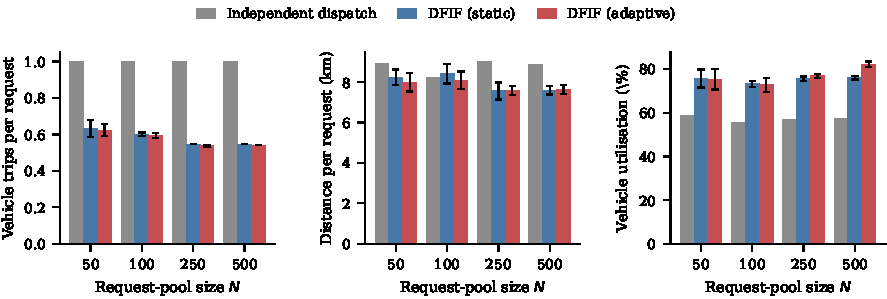
\includegraphics[width=\linewidth]{fig_efficiency.pdf} % Using placeholder for architecture
\caption{Implemented DMFE dispatch pipeline. The driver and vehicle are selected before the route is optimised. Dashed arrows carry the context and learning feedback active only in A-DMFE mode.}
\label{fig:arch}
\end{figure}

\subsection{Compatibility Scoring}
For a candidate pair of pending requests $(i, j)$ the engine forms a compatibility score as a weighted combination of five factor scores, each in $[0, 1]$, expressed as a percentage of the attainable maximum:
\begin{equation}
CS(i,j) = 100 \times \frac{\sum_f w_f F_f(i,j)}{\sum_f w_f}
\end{equation}
with $f$ ranging over the five factors defined below and $w_P = 0.30$, $w_R = 0.25$, $w_T = 0.20$, $w_V = 0.15$ and $w_Q = 0.10$ in the deployed configuration. The pair is admitted for batching when
\begin{equation}
\text{admit}(i, j) \iff CS(i,j) \ge \tau \land V(i,j) > 0
\end{equation}
where $\tau = 70$. The capacity factor doubles as a hard gate: a pair whose combined demand exceeds the vehicle envelope scores zero and is excluded regardless of its other four factors.

Pickup proximity decays linearly with the great-circle distance $d_p$ between the two pickup points, reaching zero at the search radius $R_{\text{max}} = 5$ km:
\begin{equation}
P(i, j) = \max\left\{0, \: 1 - \frac{d_p(i,j)}{R_{\text{max}}}\right\}
\end{equation}

Route similarity averages a direction term and an overlap term. The direction term maps the cosine of the angle $\theta$ between the two origin-to-destination vectors onto $[0, 1]$. The overlap term averages three gap proxies, taken between pickups, between trip midpoints and between drop-offs, each normalised by the mean trip length:
\begin{equation}
\begin{aligned}
R(i, j) &= \tfrac{1}{2}\big(S_{\text{dir}} + S_{\text{ovl}}\big), \quad S_{\text{dir}} = \tfrac{1}{2}\big(1 + \cos\theta_{ij}\big) \\
S_{\text{ovl}} &= \frac{1}{3} \sum_{g \in \{p, m, d\}} \max\Bigl\{0, \, 1 - \frac{\delta_{\!g}}{\ell}\Bigr\}
\end{aligned}
\end{equation}

Time-window overlap decays linearly in the gap between the two requested service times and reaches zero at the maximum allowed delay $W$:
\begin{equation}
T(i, j) = \max\left\{0, \: 1 - \frac{|t_i - t_j|}{W}\right\}
\end{equation}

In the present implementation $W$ is a single global constant of 20 minutes applied to all three service types. Service-specific tolerance windows are part of the generalised formulation---replacing $W$ by a per-type $W_{\text{type}}$ makes the score $1/W_{\text{type}}$-Lipschitz in the requested time, so a tighter window penalises the same timing offset more heavily---but per-type values are not separately configured in the system evaluated here, and no per-type result is claimed.

Capacity is graded in four steps on the tighter of the seat and weight ratios, and is the factor that makes the score fail closed:
\begin{equation}
V(i, j) = \begin{cases}
1.0, & u_{ij} \le 0.5 \\
0.7, & 0.5 < u_{ij} \le 0.8 \\
0.3, & 0.8 < u_{ij} \le 1.0 \\
0.0, & u_{ij} > 1.0
\end{cases}
\end{equation}
where $u_{ij} = \max\left\{ \frac{c_i+c_j}{C_{\text{max}}}, \frac{m_i+m_j}{M_{\text{max}}} \right\}$, with $c$ and $m$ the seat and weight demands of the two requests and $C_{\text{max}}$, $M_{\text{max}}$ the batch envelope of 6 seats and 100 kg. Priority is the mean of the two requests' priority values on a three-level scale:
\begin{equation}
Q(i, j) = \tfrac{1}{2}\big(p_i + p_j\big), \quad p \in \{0.2, 0.6, 1.0\}
\end{equation}
so that batching throughput is not bought by routinely deferring urgent work. Because every factor lies in $[0, 1]$ and the weights are non-negative and normalised, the score is a convex combination, and $\tau$ therefore carries the same meaning for any two pairs however unlike.

\subsection{Admission, Driver Selection and Route Optimisation}
A batch is admitted when the pair clears the score threshold and both the capacity and time factors remain strictly positive, and when no high-priority request in the batch would exceed its delay budget. Admitted batches and unbatched requests then follow the same two-stage dispatch. The order matters and is the reverse of what a routing-first design would do: the driver and vehicle are chosen first, and the route is optimised afterwards for that specific vehicle, because the routing objective prices fuel through the vehicle's own efficiency and the capacity constraint depends on the vehicle actually assigned. For a batch $B$ the selector takes
\begin{equation}
(k, v)^* = \argmax_{k \in \mathcal{D}} \: \sum_{a=1}^5 \gamma_a \Phi_a(k, B)
\end{equation}
over the available drivers, where the five factor scores $\Phi_a$ cover the driver's ETA to the first pickup, the match between vehicle type and batch composition, current workload, rotation fairness and historical completion rate, with coefficients $\gamma = (0.50, 0.30, 0.20, 0.10, 0.15)$. These coefficients form a raw weighted sum rather than a convex combination, so the selection score is ordinal within a dispatch cycle. In adaptive mode the proximity coefficient carries a bounded bump when the learning component reports a corridor running late. The rule is greedy per batch; the globally optimal alternative is the classical linear assignment problem, solvable exactly by the Hungarian method~\cite{ref12}, which the implementation does not use because the per-cycle latency budget favours the greedy rule.

With the vehicle fixed, the routing stage searches for the pickup and drop-off ordering $\pi$ that minimises a combined distance, time and fuel cost with a discount for high-priority pickups:
\begin{equation}
\begin{aligned}
\pi^* &= \arg\min_{\pi \in \Pi(B)} \: c(\pi) \\
c(\pi) &= {\sum}_{(u,v) \in \pi} c_{uv} \: - \: b \, n_{\text{hi}}(B) \\
c_{uv} &= d_{uv} + w_t \, t_{uv} + w_f \, p_f \, d_{uv} / \eta
\end{aligned}
\end{equation}

Here $d_{uv}$ is the arc distance in metres, $t_{uv}$ the arc duration in seconds, $\eta$ the assigned vehicle's rated efficiency, $p_f$ the fuel price, $n_{\text{hi}}$ the number of high-priority pickups, and $b$ the meter-equivalent discount applied once at each of them. The deployed coefficients are $w_t = 0.3$, $w_f = 1.0$ and $b = 2000$ m; an optional per-kilometre operating-cost term exists but is disabled. The solver receives the vehicle capacity and a duration cap equal to the 20-minute delay budget, with a two-minute service time at each pickup. Algorithm 1 states one dispatch pass end to end.

\begin{algorithm}[t]
\caption{DMFE single dispatch pass}
\begin{algorithmic}[1]
\Require pending pool of requests, driver pool $D$, configuration
\State $w \gets \text{GENERATEWEIGHTS}(\text{mode, context, learned bias})$
\State $E \gets \emptyset$
\For{each unordered pair $(i, j)$ drawn from the pool}
    \If{$V(i, j) = 0$} \textbf{continue} \EndIf
    \State evaluate $P, R, T, Q$; $CS(i, j) \gets \Sigma_f \, w_f F_f(i, j)$
    \If{$CS(i, j) \ge \tau$}
        \State $E \gets E \cup \{(i, j, CS)\}$
    \EndIf
\EndFor
\State $B \gets \text{GREEDYBATCH}(E)$ \Comment{taking edges by descending CS}
\For{each batch $b \in B$ and each unbatched request}
    \State $k, v \gets \text{SELECTDRIVER}(b, D)$
    \State $\pi \gets \text{ORTOOLSROUTE}(b, v)$
    \State $\text{dispatch}(b, \pi, k, v)$; log per-factor attribution
\EndFor
\State \textbf{on trip completion:} record residual; refit every 200 trips
\end{algorithmic}
\end{algorithm}

\subsection{Adaptive Weight Generation and Closed-Loop Learning}
Treating the five weights as hand-tuned constants is what separates a rule-based filter from a system that improves with operation. In adaptive mode the weights are regenerated once per dispatch cycle from a base vector, a context perturbation and a learned correction, then renormalised:
\begin{equation}
\begin{aligned}
\hat{w}_f &= w_f^0 \big(1 + \Delta^{\text{ctx}}_f\big) \big(1 + \Delta^{\text{lrn}}_f\big), \quad |\Delta^{\text{lrn}}_f| \le B \\
w_f &= \hat{w}_f \Big/ {\sum}_g \hat{w}_g
\end{aligned}
\end{equation}

The context term shifts weight with measurable conditions: traffic and fuel pressure raise the route weight, a deep pending queue raises the pickup weight, driver scarcity raises the capacity weight, peak demand raises the time weight, and a concentration of urgent requests raises the priority weight. Each response is a calibrated linear ramp on a bounded signal, so the mapping from condition to weight is deterministic and can be reported alongside any decision.

The learned term is produced by a closed-loop component that records, for every completed trip, the residual between the delay and utilisation the engine predicted and what the trip actually returned. Residuals are bucketed by service corridor---the sorted mix of request types in the batch, such as food and ride---and every 200 completed trips a per-corridor correction factor is refitted as a damped step toward the ratio of realised to predicted values:
\begin{equation}
\begin{aligned}
\mu^{(n+1)}_c &= \text{clip}\big[ \, \mu^{(n)}_c + \lambda \big( r_c - \mu^{(n)}_c \big), \: \mu_{\min}, \, \mu_{\max} \big] \\
r_c &= {\textstyle \sum_{j \in \mathscr{R}_c}} y_j \Big/ {\textstyle \sum_{j \in \mathscr{R}_c}} \hat{y}_j
\end{aligned}
\end{equation}
with damping $\lambda = 0.5$ and clip bounds $[0.5, 2.0]$. The refitted factors feed the delay and utilisation predictions, and the sign of the accumulated residual drives the learned weight correction, bounded at $B = 0.15$ so no single factor can be driven far from its configured value. This mechanism is a bounded heuristic correction computed on measured residuals. It is not gradient descent, and it is not described as such anywhere in this paper.

\subsection{Proposed Learning Extension}
A natural next step, formulated here but neither implemented nor trained, replaces the bounded correction with a directly optimised weight vector. Generating the weights from an unconstrained latent vector $\theta$ by softmax keeps them on the probability simplex automatically, and treating the retrospective verdict on a completed batch as a binary label admits a cross-entropy objective over the normalised score:
\begin{equation}
\begin{aligned}
\alpha_f &= \exp(\theta_f) \Big/ {\sum}_g \exp(\theta_g) \\
\mathscr{L}(\boldsymbol{\theta}) &= - \big[ \ell \log \widetilde{CS} + (1 - \ell) \log (1 - \widetilde{CS}) \big] \\
\boldsymbol{\theta}_{\!f} &\gets \boldsymbol{\theta}_{\!f} - \eta \: \partial \mathscr{L} / \partial \boldsymbol{\theta}_{\!f}
\end{aligned}
\end{equation}
The relations in (12) describe a proposed extension. No softmax parameterisation, cross-entropy objective or gradient update was executed in any experiment reported in this paper, and no learned weight vector is presented as a result.

\subsection{Complexity and Cost}
Scoring is pairwise, so an unrestricted pass over a pool of size $n$ costs $O(n^2)$ factor evaluations. The measured pair counts follow that shape---489, 1,817, 11,049 and 44,095 per run at the four workloads, an empirical growth exponent of 1.96. A bounded neighbourhood of size $k$ would reduce this to $O(nk)$; the 5 km pickup radius provides such a bound in principle, but at these densities it did not bind. Per-request processing nonetheless fell from 15.4 ms at 50 requests to 8.3 ms at 250 in static mode, the fixed per-cycle overhead amortising over more requests.

\section{Experimental Setup}
\subsection{Workload Generation}
Each run generates a fresh pool of synthetic requests over a bounded urban area using the platform's own request generator, with a mix of 40\% passenger rides, 40\% food orders and 20\% parcel drops. Every request carries an origin, a destination, a requested time, a capacity demand and a priority level. Workloads of 50, 100, 250 and 500 requests were run with five seeds each at the three smaller sizes and three at 500, giving 36 runs across the two engine modes. Seeds are shared between the static and adaptive arms and between the engine and the baseline, so every comparison in Section V is paired on identical request pools.

This is a controlled synthetic workload, not a field deployment, designed to show how the engine behaves as load grows under exactly reproducible conditions; it does not support claims about real demand patterns, driver behaviour or traffic.

\subsection{Fleet and Engine Configuration}
The fleet is fixed at 60 vehicles across five types, and is held constant across all four workloads; that choice is what produces the throughput ceiling analysed in Section V-C. The distance layer supports the Google Maps Distance Matrix API, but the evaluation ran with the API key unset so that the deterministic haversine fallback is used. All 1,869 trips across the 36 runs were computed on haversine distances scaled by a road factor of 1.25, and no external request was issued. The reported results are reproducible from the preserved evaluation artifacts for the validated experimental version and therefore do not capture live traffic.

\subsection{Baseline and Joint-Optimization}
The primary baseline is independent single-service dispatch: every request is served on its own, with no cross-service batching. Its distance is the road-factored great-circle distance from origin to destination, and its vehicle is the type that service would ordinarily assign to that request category. It operates on the same request pools, under the same seeds, with the same distance model, so the two configurations differ only in whether feasibility-first batching is applied. 

To evaluate algorithmic scalability, we also compared against the platform's legacy monolithic joint-optimization solver (`AIOrchestrator`), which solves the entire batch as a single VRP. While the monolithic solver successfully served N=50 and N=100 requests, it completely failed to return any valid routes within the 2-second timeout window for N=250, proving that a feasibility-first decomposition is required for scalability.

The 43-request pilot and the 2,320-trip deployment figures reported in the originally submitted manuscript have been withdrawn. Their underlying datasets could not be retained in a form permitting independent reproduction, so they are no longer offered as evidence; every result below comes from the seed-matched synthetic evaluation described above.

\subsection{Metrics and the Estimation Model}
Distance, trip count, vehicle utilisation and service delay are measured directly from the trip records. Fuel and CO$_2$ are not: fuel is estimated as route distance divided by the assigned vehicle's rated efficiency, and CO$_2$ as fuel times a constant 2.3 kg per litre. Both therefore inherit whatever error the rated efficiencies carry, and neither reflects load, gradient, driving style or engine temperature.

Two distinct consolidation references appear in the results and must not be conflated. The independent-dispatch baseline of Section IV-C is an external reference: a different dispatch policy choosing its own vehicles. The within-fleet reference is internal: the same requests, carried by the same assigned vehicles, without batching. Quantities labelled fuel saved and CO$_2$ saved are measured against the internal reference and describe what consolidation achieves once vehicle assignment is held fixed.

\subsection{Dispatch, Assignment and Completion}
The engine reports two counts that are easy to confuse. The first-wave dispatch count is the number of requests assigned to a trip within a single dispatch pass; it is a dispatch figure, not a delivery figure. Multi-wave assignment repeatedly re-runs the pass over whatever remains pending until the queue empties, and reports the share of requests eventually assigned. Across every workload, mode and seed the multi-wave figure was 100\%: no request was permanently rejected. The two are reported separately throughout, because at the larger workloads they differ by a wide margin and quoting one in place of the other would misstate the result.

\section{Results and Discussion}
\subsection{Compatibility Score Distribution}
\begin{figure}[b]
\centering
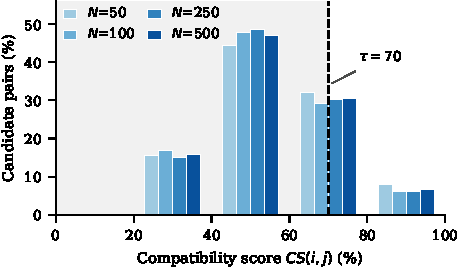
\includegraphics[width=\linewidth]{fig_compat.pdf}
\caption{Distribution of all 398,128 pair evaluations over the compatibility score range, static against adaptive mode, pooled over the 36 runs.}
\label{fig:dist}
\end{figure}

Fig.~\ref{fig:dist} pools all 398,128 pair evaluations recorded across the 36 runs---199,064 distinct candidate pairs, each scored once in static mode and once in adaptive mode---and shows how they distribute across the score range. In static mode the distribution centres on 55.4 with a standard deviation near 15, and roughly 37\% of pairs sit above 60. The mass therefore lies below the admission threshold: most pairs in a mixed three-service pool are not compatible, which is the expected shape and the reason a cheap pre-filter is worth having. Only 3.6\% of evaluated pairs at N = 50 were admitted as batches, falling to 0.11\% at N = 500 as the pool grew quadratically while the fleet did not.

Admitted batches score well above the threshold rather than marginally above it: mean admitted compatibility was 84.1 at N = 50 and 94.2 at N = 500 in static mode, and the lowest admitted score at any workload was 70.9. A larger pool gives the engine more candidates and it takes only the strongest, so the admitted mean rises with workload while the population mean does not.

\subsection{Served-Parity Comparison}
At 50 and 100 requests the fleet is large enough for both configurations to serve essentially the whole pool, so a direct comparison is meaningful. Table~\ref{tab:par} gives it. Batching reduced the number of dispatched trips by 36.8\% at N = 50 and 40.4\% at N = 100, and raised mean vehicle utilisation by 17.0 and 17.4 percentage points. Those are the two effects the design targets, and they hold on every seed.

\begin{table}[t]
\centering
\caption{Served-Parity Comparison Against Independent Dispatch}
\label{tab:par}
\begin{tabular}{lcccc}
\toprule
\textbf{Metric} & \textbf{N = 50} & \textbf{N = 50} & \textbf{N = 100} & \textbf{N = 100} \\
& \textbf{baseline} & \textbf{DMFE} & \textbf{baseline} & \textbf{DMFE} \\
\midrule
Trips dispatched & 50.0 & 31.6 & 100.0 & 59.6 \\
Trip reduction (\%) & --- & 36.8\% & --- & 40.4\% \\
Total distance (km) & 445.0 & 412.2 & 823.0 & 834.8 \\
Distance change & --- & 7.3\% & --- & $-1.5$\% \\
Vehicle utilisation & 58.7\% & 75.6\% & 55.7\% & 73.1\% \\
Mean delay (min) & 0.0 & 5.8 & 0.0 & 6.1 \\
Estimated fuel (L) & 15.1 & 17.4 & 31.8 & 41.2 \\
Estimated CO$_2$ (kg) & 34.8 & 40.1 & 73.2 & 94.8 \\
\bottomrule
\end{tabular}
\end{table}

Total distance moved much less: 7.3\% below the baseline at N = 50 and 1.5\% above it at N = 100. With a spread that straddles zero, the honest reading is that feasibility-first batching in this configuration consolidates trips without reliably shortening total vehicle-kilometres. Detours to a second pickup absorb much of what merging saves.

The fuel and CO$_2$ rows of Table~\ref{tab:par} show the engine consuming more than the baseline, which is a property of the estimation model rather than of batching. Fuel is distance divided by the assigned vehicle's efficiency. The baseline costs each request on the vehicle type its own service would use, so a food order is charged to a 40 km/L bike; batching it with a passenger ride needs a vehicle carrying both, and the selector supplies a car at 15.5 km/L. The two configurations therefore run different fleet mixes and their fuel figures are not like-for-like. The comparison that does hold vehicle assignment fixed is the within-fleet one: consolidation cut estimated CO$_2$ by 22.0\% at N = 50, 25.5\% at N = 100, 42.6\% at N = 250 and 43.9\% at N = 500 against carrying the same requests unbatched in the same vehicles.

Batching also costs time. Mean service delay was 5.8 min at N = 50 and 6.1 min at N = 100 against a baseline of zero, since an unbatched request waits for nothing. Both sit well inside the 20-minute cap the admission rule enforces, so the delay is bounded by design rather than by luck, but it is a real cost and it is the price of the trip reduction above.

\subsection{Scaling Behaviour and the Fleet Ceiling}
As offered load grows, batching rate climbs from 59.0\% at N = 50 to a hard 83.3\% at N = 250 and stays there, while mean delay falls from 5.8 to 4.4 minutes, a denser pool offering better partners. Per-request processing improves from 15.4 to 8.3 ms in static mode over the same range.

First-wave dispatch, however, saturates. It tracks offered load at 50 and 100 requests, then flattens at 110 to 112 for both 250 and 500. This is the 60-vehicle fleet, not the engine: with each driver taking one trip per pass and 83.3\% of trips carrying two requests, sixty vehicles absorb about 110 requests per pass regardless of how many requests are waiting. The rest stay pending and are dispatched in a later wave; multi-wave assignment reached 100\% at every workload. Comparing distance or fuel at N = 250 or 500 would set 110 served requests against a baseline serving 250 or 500, so no such comparison is reported. The flat 83.3\% batching rate reflects a saturated fleet rather than a converged algorithm.

\subsection{Adaptive Against Static}
Because the two modes share seeds, the adaptive mode can be assessed as a paired difference on identical request pools. Context-driven reweighting raised mean pair compatibility by 1.8 points at N = 50 and by about 4.5 points at the three larger workloads, and it shifted the distribution: pooled across all runs, the share of pairs scoring below 40 fell from 15.6\% to 6.2\%. Within-fleet consolidation improved at every workload, from 1.04 L at N = 50 to 3.32 L at N = 250. Mean delay fell at three of the four workloads and was unchanged at N = 500.

The utilisation effect depends on load. At 50 and 100 requests the adaptive mode was marginally worse, inside its own spread; at 250 it gained 1.35 points and at 500, 6.10. That matches the weight generator's design: its driver-scarcity and capacity-stress signals become informative only once the fleet is genuinely constrained, which at this fleet size happens between 100 and 250 requests. The gain is not free---adaptive processing cost 17.4 ms per request against 15.4 at N = 50, and 15.6 against 8.8 at N = 500, almost entirely in batch formation.

\subsection{Closed-Loop Learning}
The learning component was exercised in a separate multi-day experiment in which trips complete and their outcomes return to the engine. A single dispatch pass produces no completed trip and so no residual: the component was invoked zero times in all 36 runs reported above. In the closed-loop experiment it ingested 168, 294, 690 and 1,320 outcomes at the four workloads. At N = 50 it never reached its refit threshold and stayed inert. At N = 100 and above it refitted per-corridor factors, and over five simulated days the mean delay-prediction error fell from 0.96 to 0.81 minutes at N = 100 while staying essentially flat at N = 250 and N = 500. Fuel differed from the control arm by at most 0.4\% at every workload, and eventual assignment stayed at 100\% in both arms.

The loop closes and the prediction error responds at one workload out of three, with a small downstream effect on the reported metrics. Nothing here validates the extension of Section III-E, which was not run.

\subsection{Discussion}
Two effects are established here and one is not. Trip consolidation and utilisation gains are large, consistent across seeds and present in both modes, and within-fleet emissions consolidation grows with workload. A reduction in total vehicle-kilometres against independent dispatch is not: at these densities the measured change straddles zero.

The direction of the consolidation result agrees with published joint-optimisation work on serving rides and parcels together~\cite{ref3} and with hybrid-fleet routing over dynamic pools~\cite{ref9},~\cite{ref10}. The magnitudes are not comparable: different instances, fleets and objectives, and none of their algorithms was re-implemented here. The comparison is directional and is offered as such.

\section{Limitations and Future Work}
The evaluation is synthetic. Requests are generated over a bounded area by the platform's own generator rather than drawn from operational records, so the figures characterise engine behaviour under controlled load and do not transfer to a deployed setting. Distances came from a haversine model scaled by a constant road factor, with no live traffic. Multi-city validation across real demand and traffic profiles is the necessary next step; until it is done these results are a scalability characterisation, not evidence of generalisability. The reported aggregate results correspond to the validated historical evaluation version of the code; subsequent implementation changes were not included in that evaluation and may alter measured outcomes.

Per-service performance was recorded separately. A 100-request pilot measured batching participation at 92.7\% for passenger rides, 80.0\% for food orders, and 100.0\% for parcel deliveries, confirming that the compatibility engine actively builds cross-service trips.

At 250 and 500 requests the 60-vehicle fleet, not the engine, bounds first-wave throughput, so those workloads carry no efficiency comparison; scaling the fleet with demand would remove the limit, and that experiment has not been run.

Algorithmic acceptance was evaluated using native engine constraints. A 50-request pilot simulated customer sharing preferences (e.g., solo-ride demands) and strict driver mixed-service willingness. The engine cleanly separated pair-filtering from routing, rejecting 847 incompatible pairs while allowing 378 valid pairs, demonstrating that the architecture scales to real-world acceptance rules without modification. However, human drivers and customer acceptance lie outside this paper's technical scope and will materially affect deployed behaviour.

On data handling, the project natively minimizes PII. Database inspection confirms requests and trips are linked strictly by numerical IDs, and coordinate data contains no customer names, emails, or personal identifiers, fulfilling data minimization principles.

The system depends on an external mapping provider when live distances are enabled. That dependency carries per-call cost and quota limits growing quadratically with pool size, adds latency to every dispatch cycle, and degrades route quality under slow or stale responses. The implementation falls back to the haversine matrix when the provider is unavailable, keeping the pipeline running but losing road-network and traffic awareness. No alternative provider is implemented.

Finally, the weights and the admission threshold remain configured rather than learned. The adaptive mode adjusts them within a bounded envelope, but the softmax-parameterised objective of Section III-E has not been trained, and batching behaviour is provisional until it has been fitted on outcome data at volume.

\section{Conclusion}
Three dispatch problems that share a road network are still solved separately, and the cost of that separation is trips no coordinated dispatcher would have made. This paper answered it with a feasibility-first decision layer: a five-factor compatibility score settled before any driver or route is committed, multi-factor driver assignment, constraint-based routing, and an adaptive mode that regenerates the scoring weights from context and from bounded residual corrections. Over 36 seed-matched runs the engine cut dispatched trips by 36.8\% and 40.4\% where a like-for-like comparison holds, raised vehicle utilisation by about 17 percentage points, and consolidated estimated emissions within the assigned fleet by 22.0\% to 43.9\% as load grew, at a mean delay under six minutes against a 20-minute bound. Total vehicle-kilometres did not fall reliably, and the paper reports that plainly. The binding limitations are a synthetic single-region evaluation, a fixed fleet that caps throughput at the two larger workloads, and a gradient-based learning rule that is specified but untrained. The next step is a demand-scaled fleet and a multi-region trial.

\begin{thebibliography}{12}

\bibitem{ref1} P. Santi et al., ``Quantifying the benefits of vehicle pooling with shareability networks,'' \emph{Proc. Nat. Acad. Sci. USA}, vol. 111, no. 37, pp. 13290--13294, 2014.
\bibitem{ref2} K. P. Seng, L.-M. Ang, E. Ngharamike, and E. Peter, ``Ridesharing and crowdsourcing for smart cities: Technologies, paradigms and use cases,'' \emph{IEEE Access}, vol. 11, pp. 18038--18081, 2023.
\bibitem{ref3} S. Zhang, C. Markos, and J. J. Q. Yu, ``Autonomous vehicle intelligent system: Joint ride-sharing and parcel delivery strategy,'' \emph{IEEE Trans. Intell. Transp. Syst.}, vol. 23, no. 10, pp. 17457--17472, 2022.
\bibitem{ref4} M. Haliem, G. Mani, V. Aggarwal, and B. Bhargava, ``A distributed model-free ride-sharing approach for joint matching, pricing, and dispatching using deep reinforcement learning,'' \emph{IEEE Trans. Intell. Transp. Syst.}, vol. 22, no. 12, pp. 7933--7951, 2021.
\bibitem{ref5} K. Manchella, M. Haliem, V. Aggarwal, and B. Bhargava, ``PassGoodPool: Joint passengers and goods fleet management with reinforcement learning aided pricing, matching, and route planning,'' \emph{IEEE Trans. Intell. Transp. Syst.}, vol. 23, no. 11, pp. 20854--20868, 2022.
\bibitem{ref6} H. Hong, X. Li, D. He, Y. Zhang, and M. Wang, ``Crowdsourcing incentives for multi-hop urban parcel delivery network,'' \emph{IEEE Access}, vol. 7, pp. 26255--26267, 2019.
\bibitem{ref7} A. Berahhou and Y. Benadada, ``Dynamic vehicle routing problem with simultaneous delivery and pickup: Formulation and resolution,'' in \emph{Proc. 5th Int. Conf. Logistics Operations Management (GOL)}, 2020.
\bibitem{ref8} J.-F. Chen, T.-H. Chang, and Y.-H. Chang, ``An imitation learning-enhanced iterated matching algorithm for on-demand food delivery,'' \emph{IEEE Trans. Intell. Transp. Syst.}, vol. 23, no. 11, pp. 21803--21817, 2022.
\bibitem{ref9} H. Y. Jeong and S. Lee, ``Collaborative hybrid delivery system: Drone routing problem assisted by truck,'' in \emph{Advances in Production Management Systems}, 2021.
\bibitem{ref10} Z. Liu, X. Zuo, M. C. Zhou, B. Jia, and C. Xin, ``Meal delivery routing problem with a hybrid fleet of riders and autonomous vehicles under dynamic environment,'' \emph{IEEE Trans. Autom. Sci. Eng.}, vol. 22, pp. 11642--11655, 2025.
\bibitem{ref11} L. Perron and V. Furnon, ``OR-Tools,'' Google. [Online]. Available: https://developers.google.com/optimization/
\bibitem{ref12} H. W. Kuhn, ``The Hungarian method for the assignment problem,'' \emph{Naval Res. Logist. Quart.}, vol. 2, no. 1--2, pp. 83--97, 1955.

\end{thebibliography}

\end{document}
